\def\DevnagVersion{2.15}\documentclass[11pt]{article}
\usepackage{acl2014}
\usepackage{times}
\usepackage{url}
\usepackage{latexsym}
\usepackage{devanagari}
\usepackage{graphicx,subfigure}
\usepackage{float}
\usepackage{pdfpages}


%\setlength\titlebox{5cm}



\title{Word vector models for Hindi: A  Sentiment Analysis evaluation}

\author{Pranjal Singh \\
  Dept. of Computer Science \& Engg. \\
  IIT Kanpur \\
  {\tt spranjal@iitk.ac.in} \\\And
  Amitabha Mukerjee \\
  Dept. of Computer Science \& Engg. \\
  IIT Kanpur \\
  {\tt amit@cse.iitk.ac.in} \\}
\date{}

\begin{document}
\maketitle
\begin{abstract}
In recent years, distributional semantics or word vector models
have been proposed to capture both the syntactic and semantic similarity
between words.  Since these can be obtained in an unsupervised manner, they
are of interest for under-resourced languages such as Hindi.  We test the
efficacy of such an approach for Hindi, first by a subjective overview which
shows that a reasonable measure of word similarity seems to be captured
quite easily.  We then apply it to the sentiment analysis for
two small Hindi databases from earlier work.  In order to
handle larger strings from the word vectors, 
several methods - additive, multiplicative, or tensor neural
models, have been proposed.  Here we find that even the simplest - an additive
average, results in an impressive
accuracy gain on state of the art by 10\% (from 80\%) for
two review datasets.  The results suggest that
it may be worthwhile to explore such methods further for Indian languages.
\end{abstract}


\section{Introduction}
Over a period of nearly a millenium, Indian grammarians have been trying to find whether sentence meaning accrues by combining word
meanings, or whether words gain their meanings based on the context they
appear in~\cite{Matilal:90}.  The former position, that
meaning is {\em compositional}, has been associated with the fregean
enterprise of semantics, whereas recent models, building on large corpora of
text (and associated multimedia) a large degree of success has accrued to
models that attempt to model word meaning based on their linguistic context
(e.g. ~\cite{Landauer:97}).  The latter line has resulted in strong improvements in several NLP tasks using word vectors~\cite{Collobert:08,Turian:10,Mikolov:13a,Socher:13}. 
The advantage of these approaches is that they can capture both the syntactic
and the semantic similarity between words in terms of their projections onto
a high-dimensional vector space; further, it seems that one can tune the
privileging of syntax over semantics by using local as opposed to large contexts~\cite{Huang:12}. 

For resource-poor languages, these approaches have the added lure
that many of these methods are completely unsupervised and work directly with
large raw text corpora, thus
avoiding contentious issues such as deciding on a POS-tagset, or expensive
human annotated resources such as treebanks.  For Indian languages which are
highly inflected, stemming or identifying the lemma is another problem
which such models can overcome, provided the corpus is large enough.
Nonetheless, this approach remains under-explored for Indian languages.
At the same time, it must 
be noted that many approaches seek to improve their performance
by combining POS-tags and even parse tree structures
into the models for higher accuracies in specific tasks~\cite{Socher:13}. 

Vector models for individual words are obtained via distributional learning, the
mechanisms for which varies from document-term
matrix factorization~\cite{Landauer:97},
various forms of deep learning~\cite{Collobert:08,Turian:10,Socher:13}, 
optimizing models to explain co-occurrence constraints
~\cite{Mikolov:13a,Pennington:14},etc. Once the word vectors have been assigned, similarity between words can
be captured via cosine distances. 

One problem in this approach is that of 
combining the word vectors into larger phrases.  In past work,
inverse-similarity weighted averaging appears
to work to some extent even for complex tasks such as essay grading \cite{Landauer:03},
but multiplicative models (based on a reducing the tensor products of the
vectors) appears to correlate better with human
judgements~\cite{Mitchell:08,Socher:13}.
Another complexity in composition is that composing words across phrasal
boundaries are less meaningful than composing them within a phrase - this has
led to models that evaluate the nodes of a parse tree, so that only coherent
phrases are
evaluated~\cite{Socher:13}. 
The results reported here, are based on applying the Skip-Gram  model~\cite{Mikolov:13b} to Hindi. 

\subsection{Sentiment Analysis}

In order to evaluate the efficacy of the model, we apply it to the task of
sentiment analysis.
Here the problem is that of identifying the polarity of sentences (Liu et
al. 2012); for example: 
\begin{itemize}
\item Positive: {\dn rA\8{m} n\? khAnF kF r\327wtAr khF{\qva} Tmn\? nhF{\qva} dF} [Ramu didn't allow the pace of the story to subside]
\item Negative: {\dn pd\?{\qvb} pr EdKAyA jA rhA KO\327w Esn\?mAGr m\?
nhF{\qva} psr pAtA} [The horror shown on the screen didn't reach the theater]
\end{itemize}

This is a problem that has attracted reasonable attention in Hindi (see section~\ref{sec:related}), since most sentiment
analysis is oriented towards semantics, and one may bypass the syntactic
processing which remains poor for Hindi.   Methods that have been used
are largely based on assigning a sentiment effect for individual words, and
then combining these in some manner to come up with an overall sentiment for
the document.  Such methods ignore word order and have been
criticized since the import of a sentence can change completely simply by
re-arranging the words, though the sentiment evaluation remains the same.
Several groups have attempted to improve the situation by modeling
the composition of words into larger contexts~\cite{Mikolov:13c,Socher:13,Johnson:14,baroni-bernardi-14_frege-in-space-distributional-semantics}.
However, most of the work on sentiment analysis in Hindi has not attempted to
form richer compositional analyses.   For the type of corpora used here, the 
best results, obtained by combining a sentiment lexicon with hand-crafted rules (e.g. modeling negation and "but" phrases), reach an accuracy of 80\%~\cite{Mittal:13}.  

In this work, we first learn a distributional word vector model
based on the wikipedia Hindi corpus as well as the sentiment corpus, and then
we use this to discern 
the polarities on the existing corpora of movie and product reviews.
To our own surprise, we find that even a simple additive composition model
improves the state of the art in this task significantly (a gain of nearly
10\%). 
When used for the much better-researched, larger datasets of English
the system does respectably, but well behind the very best
models that attempt more complex composition models. 
So the question arises as to whether the very significant gains in
Hindi are due to some quirk in the 
dataset, or could it be that Hindi word vectors are particularly informative,
e.g. owing to more highly inflected nature of its
surface forms.  Also, if the results are not corpus-specific, it also raises
the possibility that word vector methods may result in significant gains in
other similar problems for Hindi. 
 
% For example, the sentences below give a brief idea of what positive and negative sentiment means.
% \begin{itemize}
% \item Positive: {\dn yh EPSm aQCF h\4}
% \item Negative: {\dn yh smAn b\7{h}t KrAb h\4}
% \end{itemize}
% \footnotetext{en.wikipedia.org/wiki/List\_of\_languages\_by\_number\_of\_native\_speakers}
% Majority of the existing work in this field is in English (Pang and Lee, 2008).
% Our model uses word vector averaging to build document vectors which constitute a feature set for our SVM classier. We have used skip-gram model (Mikolov et al., 2013b) for building word vectors because deep network model of Collobert et al.(2008) takes too much time for training. Also the word embeddings obtained by them are not as good as those obtained by Mikolov et al.(2013b). On NER task, skip-gram obtained F1-score of 93.1 while CW obtained F1-score of 92.2. We have also experimented with tf-idf for building our feature set. Our model shows slight improvement in performance if we filter out certain corpus based stop words. This is a first attempt to use word vectors for sentiment analysis in Hindi. Word vectors capture both semantic and syntactic information for a given corpus. Words which are semantically and syntactically related tend to be closer in high-dimensional space.\\
% This paper is organised as follows. Section 2 presents related work in the field of sentiment analysis. Section 3 describes our approach in detail. Experiment setup and datasets are described in Section 4. Section 5 looks into the results we have obtained and compares them with the results of existing models. Section 6 concludes and presents the future work.


\section{Related Work}
\label{sec:related}
Sentiment analysis is a well-known research area in NLP today (see reviews in~\cite{Liu:12} and Pang et al. (2008), and also
challenge in SemEval-2014).  Early work on movie review sentiments achieved an accuracy of 87.2\% (Pang et al. 2004) on a dataset that discarded objective sentences and used text categorization techniques
on the subjective sentences. Le and Mikolov (2014) use word vector models and obtain 92.6\% accuracy on IMDB movie review dataset.
They used distributed bag-of-words model, which they call as \emph{paragraph vector}. More difficult challenges involve short texts with nonstandard vocabularies,as in twitter.  Here, some authors focus on building extensive feature sets (e.g. Mohammad et al.(2013); F-score 89.14). \\
% WANG IS NOT BEING REFERRED TO
% Wang et al. (2014) propose a word vector neural-network model, which takes
% both sentiment and semantic information into account. This word vector
% expression model learns word semantics and sentiment at the same time as well
% as fuses unsupervised contextual information and sentence level supervised
% labels.

There has been limited work on sentiment analysis in Hindi -- see review in
~\cite{Medagoda:13}, who surveys sentiment analysis in non-English languages). Joshi et al. (2010) compared three approaches: In-language sentiment
analysis, Machine Translation and Resource Based Sentiment Analysis. By using WordNet linking, words in English SentiWordNet were replaced by equivalent Hindi words to get H-SWN. The final accuracy achieved by them is 78.1\%.

% MISSING:
% DROP:% Wang et al. (2014) 
% DROP: Mukherjee et al. (2012)
% 	mukherjee-bhattacharyya-12_sentiment-analysis-in-twitter
% 	NOT HINDI - DROP
% replace Arora etal
% 	arora-bakliwal-varma-12_hindi-subjective-lexicon_wordnet-graph
% 	[accuracy 74%]
% 	[ALSO in table 6?]
% with
% Bakliwal etal 2012 -
% 	bakliwal-arora-varma-12_hindi-subjective-lexicon-for-polarity
% 	[accuracy 79.0% after incorporating POS tag information, and focusing
% 	on adjectives / adverbs]

\cite{Bakliwal:12}
traversed the WordNet ontology to antonyms and synonyms 
to identify polarity shifts in the word space. Further
improvements were achieved by using a partial stemmer (there is no good
stemmer / morphological analyzer for Hindi), and focusing on 
adjective/adverbs (45 + 75 seed words given to the system); their 
final accuracy was 79.0\% for the product review dataset. 
% Mukherjee et al. (2012) presented the inclusion of discourse markers
% in a bag-of-words model and how it improved the sentiment classification
% accuracy by 2-4\%.  % <--- NOT HINDI
Mittal et al. (2013) incorporate hand-coded
rules dealing with negation and discourse relations and extend the
HSWN lexicon with more opinion words.  Their algorithm achieves  80.2\%
accuracy on classification of movie reviews on a separate dataset.\\

\section{Word-Vectors by using Skip-Gram}
Mikolov et al. (2013b) proposed two neural network models for building word
vectors from large unlabelled corpora; Continuous Bag of Words(CBOW) and
Skip-Gram.  In the 
CBOW model, the context is the input, and one tries to learn a vector
for the central word; in Skip grams, the 
input is the target word and one tries to guess the set of
contexts.  The Skip gram was found to 
perform better on smaller corpora, and
here we have focused on this model for building our word vectors. 
The model uses each current word as an input to a log-linear
classifier with continuous projection layer, and predict words within a
certain range before and after the current word. The objective is to maximize
the probability of the context given a word within a language model:

\begin{center} $p(c|w;\theta)=\frac{\exp^{v_c.v_w}}{\sum_{c' \in C}\exp^{v_c.v_w}}$ \end{center}
where $v_c$ and $v_w$ $\in$ $R^d$ are vector representations for context $c$ and word $w$ respectively. $C$ is the set of all available contexts. The parameters $\theta$ are $v_ci$, $v_wi$ for $w \in V$, $c \in C$, $i \in 1,....,d$ (a total of $|C| \times |V| \times d$ parameters).\\

\begin{figure}[ht!]
\centering
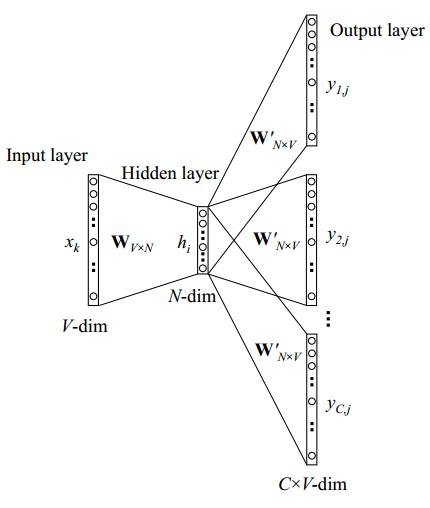
\includegraphics[width=70mm, height=70mm]{skipgram.jpg}
\caption{Skip Gram Model(Figure from Rong (2014)) \label{fig:skipgram}}
\end{figure}

%\subsection{tf-idf}
%Let $D=d_1, d_2, d_3....d_N$ be $N$ documents under study and $T=t_1, t_2, t_3,....t_M$ be the $M$ unique terms in these documents, then each document can be represented as a $M$-dimensional vector:\\
%$t_d=\{tf_1,tf_2,tf_3,...tf_M\}$\\
%$tf-idf$ weights discounts the frequency of terms based on their importance to a particular document in the entire document set collection under consideration. This is done as follows:
%\begin{center}
%$tfidf(d,t)=tf(d,t) \times \log(\frac{|D|}{df(t)})$ 
%\end{center}
%Here $df(t)$ is the number of documents in which term $t$ appears.

\subsection{Vector Averaging for phrases}
As an output of the word vector learning, we now have a $n$-dimensional
vector representation for each word in the Hindi corpus.  Now we need to
assign features for sentences and paragraphs taken from the sentiment dataset
(training and test).  Mikolov et al. (2013b) and Levy et al. (2014) show that
many relational similarities can be recovered by means of vector arithmetic
in the embedded space.  Thus, additive models are useful, though
others have claimed that multiplicative models correlate better with human
judgments~\cite{Mitchell:08,Socher:13}.  In this work, we have retained teh
simplicity of vector averaging to model larger chunks of  discourse.
This models the sentence/document in the same high dimensional space.

A preprocessing step involved removing some words that appear at very high or
very low frequencies in the corpus.  
Our model was trained on the Hindi Wikipedia dump to create vector
representations for words. The previous two vectors were concatenated to
create another feature set for training purpose.  
%?? SIZE of wikipedia corpus, number of independent words etc. 

\underline{\emph{Algorithm}}
\begin{enumerate}
%\setlength{\itemsep}{0.5pt}
\item Input the Hindi text corpus
\item Train skip-gram model to obtain word vector representation
\item Given a sentiment training set, obtain average vector data for each sentence/document
\item Obtain tf-idf vector for each sentence/document in the corpus
\item Concatenate vectors of step 3 and step 4 to obtain a feature set for a training instance
\item Train linear SVM with $m$-fold cross validation to create a classifier
(here $m$=20)
\end{enumerate}

\section{Experiment Setup}
This section describes the corpus used in our experiment along with different experiment models and parameters. In all the experiments, we did 20-fold cross validation to calculate classification accuracy using linear SVM.
\subsection{Corpus}
We experimented on two Hindi review datasets. One is the Product Review dataset (LTG, IIIT Hyderabad) containing 350 Positive reviews and 350 Negative reviews. The other is a Movie Review dataset (CFILT, IIT Bombay) containing 127 Positive reviews and 125 Negative reviews. Similarly, for English, we trained on IMDB movie review dataset (Maas et al.(2013)) which consists of 25,000 positive and 25,000 negative reviews.\\
We also trained our skip-gram model on Hindi Wikipedia text dump (approx. 290MB) containing around 24M words with 724K words in the vocabulary. This provided us with good embeddings due to larger size and contents from almost all domains.

The quality of word vectors can be evaluated by comparing them with words
which are closer to them semantically and syntactically. This is usually
done via cosine similarity.  Another evaluation can be done
through tSNE~\cite{Maaten:08} which helps in
visualization which maps each high-dimensional data point to a 
two or three-dimensional map. In our experiment, we took 5K words and plotted
them with tSNE (fig.~\ref{fig:5K_hindi_zoom}). 

\begin{figure}[ht!]
\centering
\includegraphics[width=80mm]{tsne.pdf}
\caption{t-SNE visualization of the top 5000 Hindi Words in high dimensional space.  (Magnify to see details).}
\label{fig:5K_hindi_zoom}
\end{figure}

Figure \ref{fig:5K_hindi_zoom} gives a closer look into few clusters which depicts the relation between words in high dimensional space. Figure \ref{fig:5K_hindi_zoom1} shows that words such as {\dn mO\8{j}d} and {\dn uplND} are closer to each other but farther from words such as {\dn \31EwyAdA} and {\dn aEDk}.

%\begin{figure*}[ht]
%\begin{minipage}[b]{0.31\linewidth}
%\centering
%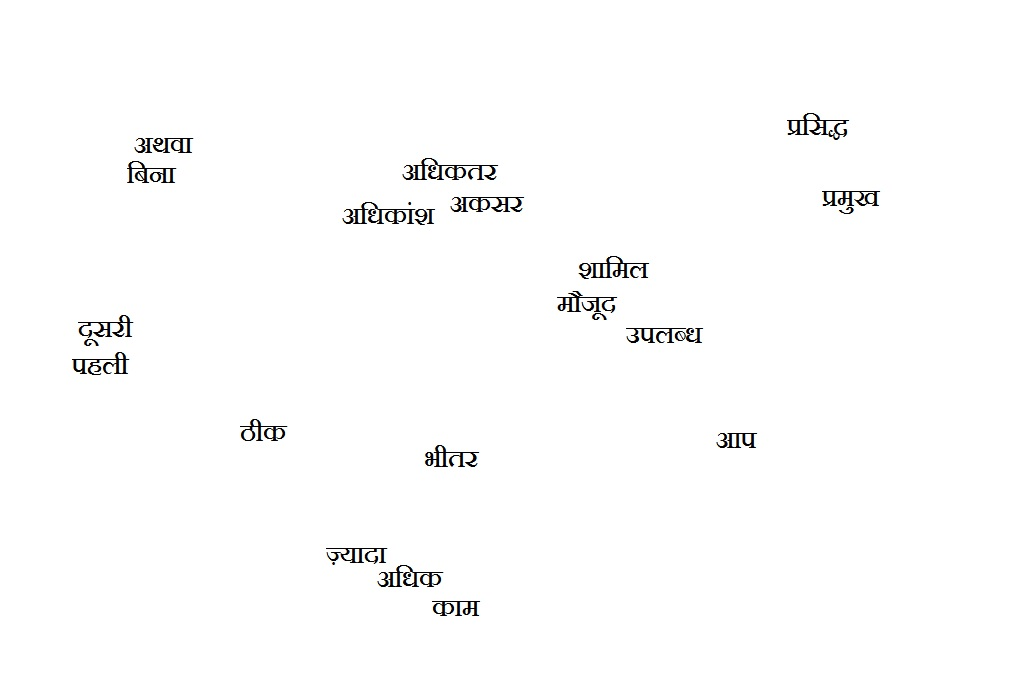
\includegraphics[width=\textwidth]{5K_hindi_zoom1.jpg}
%\caption{default}
%\label{fig:figure1}
%\end{minipage}
%\hspace{0.35cm}
%\begin{minipage}[b]{0.31\linewidth}
%\centering
%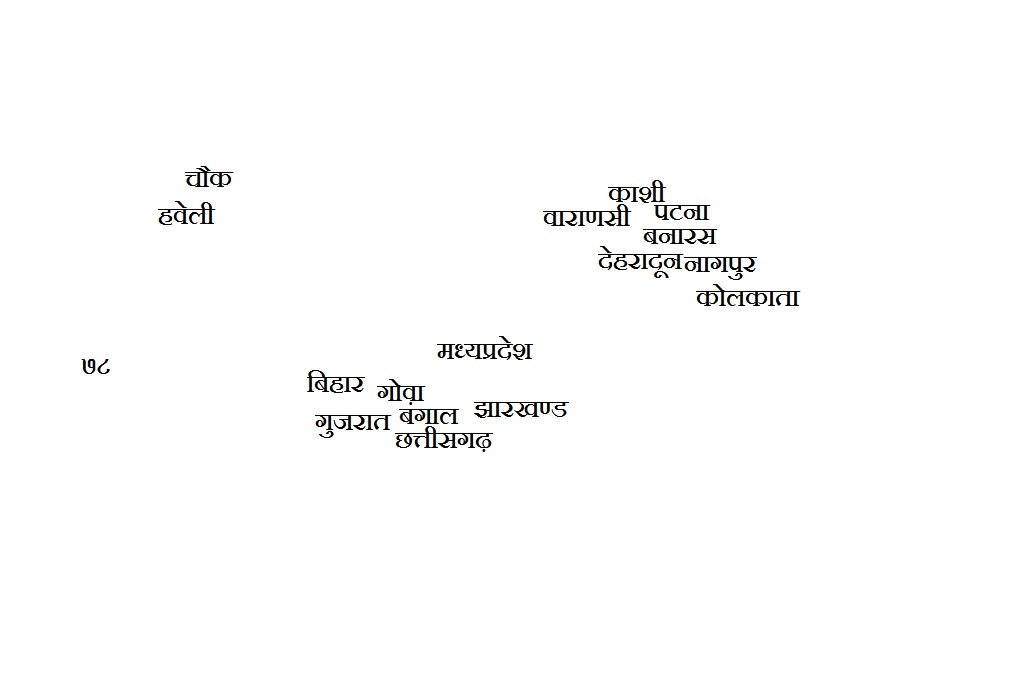
\includegraphics[width=\textwidth]{5K_hindi_zoom2.jpg}
%\caption{default}
%\label{fig:figure2}
%\end{minipage}
%\hspace{0.35cm}
%\begin{minipage}[b]{0.31\linewidth}
%\centering
%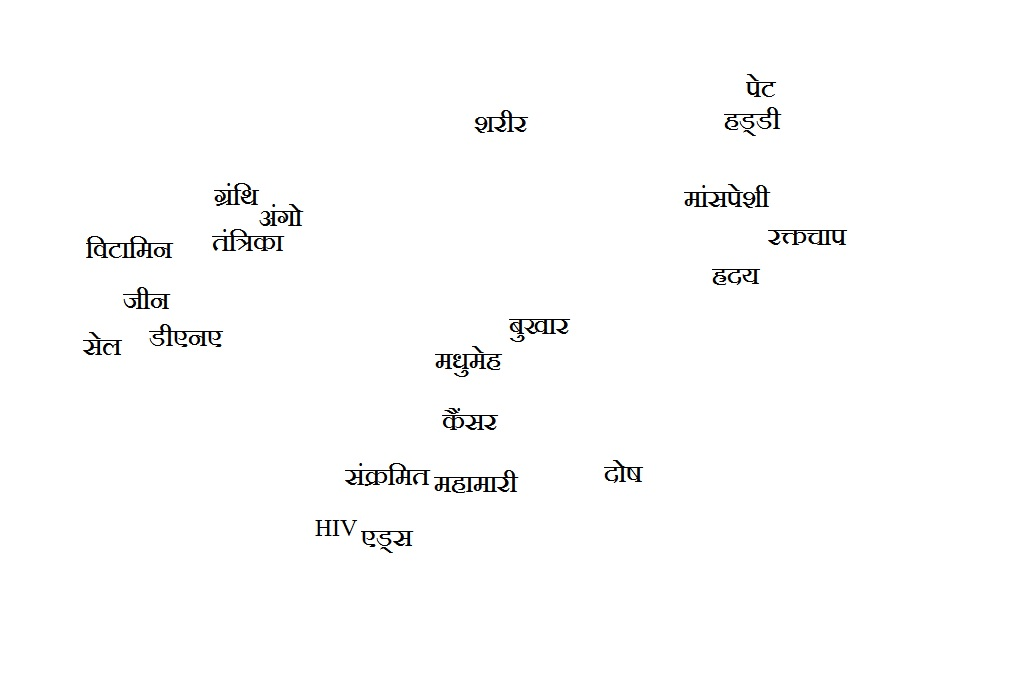
\includegraphics[width=\textwidth]{5K_hindi_zoom3.jpg}
%\caption{default}
%\label{fig:figure3}
%\end{minipage}
%\end{figure*}


\begin{figure}[ht!]
\centering
\subfigure[]{
            \label{fig:5K_hindi_zoom1}
            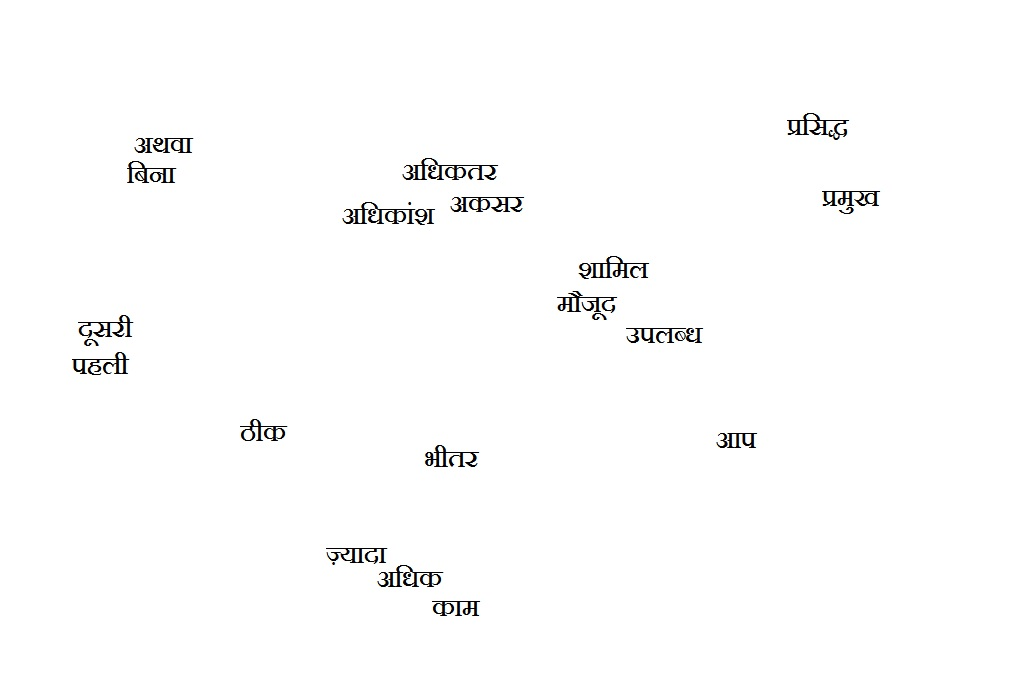
\includegraphics[width=0.4\textwidth]{5K_hindi_zoom1.jpg}
}
\subfigure[]{
            \label{fig:5K_hindi_zoom2}
            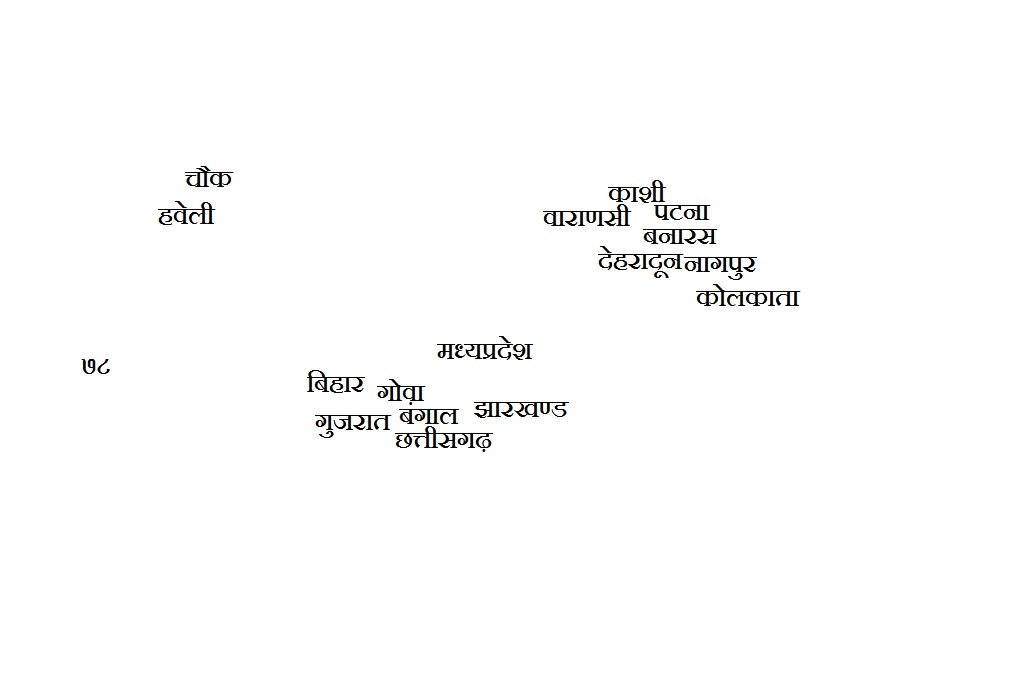
\includegraphics[width=0.4\textwidth]{5K_hindi_zoom2.jpg}
}
%\subfigure[]{
%            \label{fig:5K_hindi_zoom3}
%            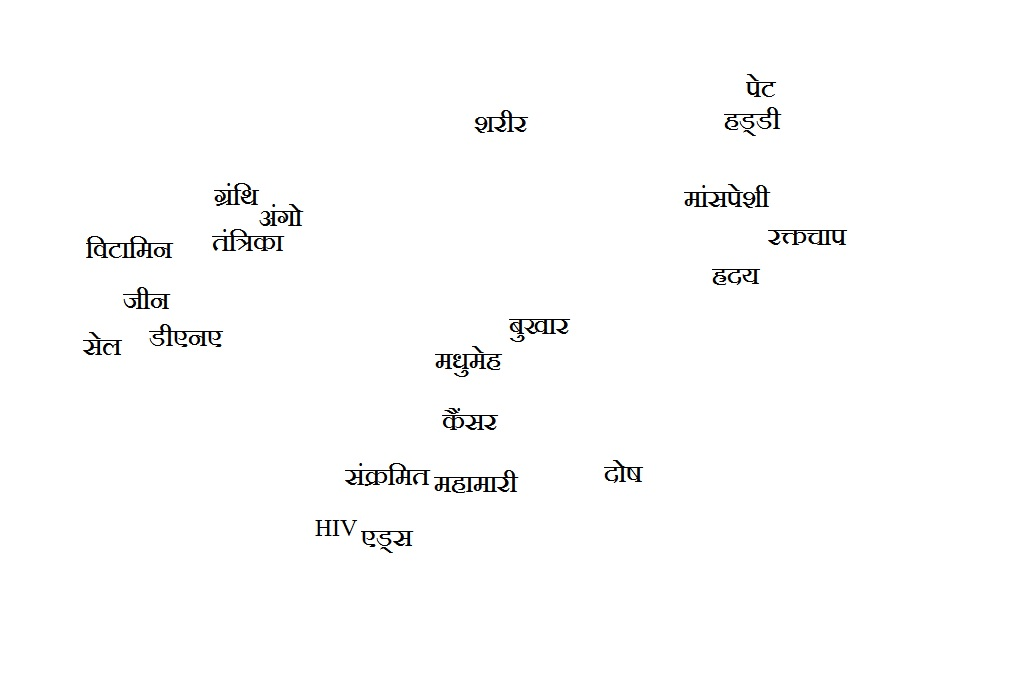
\includegraphics[width=0.4\textwidth]{5K_hindi_zoom3.jpg}
%}
\caption{A closer look at two clusters in the visualization showing a) quantity
relations and b) locations. }
\label{fig:5K_hindi_zoom}
\end{figure}


\subsection{Skip-Gram and \emph{tf-idf} based Word Vectors}
In this experiment, we first generated 300-dimensional word vectors by training skip-gram model on both review corpus. The context size was taken as 5. We then averaged-out word vectors for each document to create document vectors. This now acts as a feature set for that particular document.
We also created \emph{tf-idf} vectors for each document. This can be seen as a vector representation of that particular document. We then concatenated these document vectors with document vectors obtained after averaging-out word vector of each document. In this case, the dimension of each word vector obtained from skip-gram training was 500.

%\subsection{Skip-Gram and \emph{tf-idf} based Word Vectors without stop-words}
%In this experiment, we filtered out stop-words on the basis of their frequency in the corpus. Words which had very high or very low frequency were pruned as they had negligible contribution to the %%sentiment polarity of a document. This is a noise-reduction step and gives better results.

\section{Results}

\begin {table}[H]
\small
\begin{tabular}{ | p{5.5cm} | l | }
\hline
\textbf{Features} & \textbf{Accuracy} \\ \hline
Dredze et al.(2008) & 85.90\\ \hline
Max Entropy & 83.79\\ \hline
WordVector Averaging (Our Method) & \textbf{89.23}\\ \hline
\end{tabular}
\caption {Results on Amazon Electronics Review Dataset}
\end{table}

\begin {table}[H]
\small
\begin{tabular}{ | p{5.5cm} | l | }
\hline
\textbf{Features} & \textbf{Accuracy} \\ \hline
Maas et al.(2011) & 88.89\\ \hline
Paragraph Vector (Le and Mikolov(2014)) & 92.58\\ \hline
WordVector Averaging+Wiki (Our Method) & 87.56\\ \hline
\end{tabular}
\caption {Results on IMDB Movie Review Dataset}
\end{table}

Table 2 represents the results using three different techniques for feature set construction.
%We see that there is a slight improvement in accuracy on both datasets once we remove stop-words.
\begin {table}[H]
\small
\begin{tabular}{ | p{3cm} | l | l | }
\hline
\textbf{Features} & \textbf{Accuracy(1)} & \textbf{Accuracy(2)} \\ \hline
WordVector Averaging & 78.0 & 79.62\\ \hline
WordVector+tf-idf & 90.73 & 89.52\\ \hline
WordVector+tf-idf without stop words & \textbf{91.14} & \textbf{89.97}\\ \hline
\end{tabular}
\caption {Accuracies for Product Review and Movie Review Datasets.}
\end{table}

Table 3 and 4 compares our best method with various other methods which have performed well using techniques such as \emph{tf-idf}, subjective lexicon, etc.

\begin {table}[H]
\small
\begin{tabular}{ | p{3cm} | p{2.2cm} | l | }
\hline
\textbf{Experiment} & \textbf{Features} & \textbf{Accuracy} \\ \hline
Word Vector with SVM (Our method) & tf-idf with word vector & \textbf{91.14}\\ \hline
Subjective Lexicon (Bakliwal et al.(2012)) & Simple Scoring & 79.03\\ \hline
Hindi-SWN Baseline (Arora et al.(2013)) & Adjective and Adverb presence & 69.30\\ \hline
\end{tabular}
\caption {Comparison of Approaches: Product Review Dataset}
\end{table}


\begin {table}[H]
\small
\begin{tabular}{ | p{3cm} | p{2.1cm} | p{1.3cm} | }
\hline
\textbf{Experiment} & \textbf{Features} & \textbf{Accuracy} \\ \hline
WordVector Averaging & word vector & 78.0\\ \hline
Word Vector with SVM (Our method) & tf-idf; word vector & \textbf{89.97}\\ \hline
In language using SVM (Joshi et al.(2010)) & tf-idf & 78.14\\ \hline
MT Based using SVM (Joshi et al.(2010)) & tf-idf & 65.96\\ \hline
Improved Hindi-SWN  (Bakliwal et al.(2012)) & Adj. and Adv. presence & 79.0\\ \hline
\end{tabular}
\caption {Comparison of Approaches: Movie Review Dataset}
\end{table}

Table 5 shows the top few similar words for certain words from the corpus with cosine similarity as a distance metric. 
%The words which have higher cosine similarity tend to be semantically and syntactically related.
\begin {table}[H]
\small
\begin{tabular}{ | l | l | l | }
\hline
\textbf{{\dn aQCA}} & \textbf{{\dn{KrAb}}} & \textbf{{\dn ByAnk}} \\ \hline
{\dn b\7{h}t} & {\dn EnrAsAjnk} & {\dn By\306wkr}\\ \hline
{\dn \7{s}pr} & {\dn kM)or} & {\dn BFqZ}\\ \hline
{\dn k\?vl} & {\dn nA\7{)}k} & {\dn ByAvh}\\ \hline
{\dn itnA} & {\dn bdtr} & {\dn avsAd}\\ \hline
\end{tabular}
\caption {Some sentiment words and their neighbors}
\end{table}

\section{Conclusion and Future Work}
In this work we present an early experiment on the possibilities of distributional semantic models (word vectors) for low-resource, highly inflected languages such as Hindi.  What is interesting is that our word vector averaging method along with tf-idf results in improvements of accuracy compared to existing state-of-the art methods for sentiment analysis in Hindi (from 80.2\% to 89.9\%). \\
Distributional semantics approaches remain relatively under-explored for
Indian languages, and our results suggest that there may be substantial
benefits to exploring these approaches for Indian languages.  While this work
has focussed on sentiment classification, it may also improve a range of tasks from verbal analogy tests to ontology learning, as has been reported for other languages.   \\
In our future work, we seek to explore various compositional models - a) weighted average - where weights are determined based on cosine distances in vector space;  b) multiplicational models. Another aspect we are considering is to incorporate multiple word vectors for the same surface token in cases of polysemy - this would directly be useful for word sense disambiguation.  Identifying morphological variants would be another direction to explore for better accuracy. With regard to sentiment analysis, the idea of aspect-based models (or part-based sentiment analysis), which looks into constituents in a document and 
classify their sentiment polarity separately, remains to be explored in
Hindi.
Another point to note is that we are re-computing the word vectors
for the two review corpora, which are extremely small.  We may expect 
better performance  with a larger sentiment corpus.
%?? perhaps ASPECT requires parsing? 

We also observe that pruning high-frequency stop words improves the accuracy
by around 0.45\%. This is most likely  because such words tend to occur in
most of the documents and don't contribute to sentiment.  Similarly, words
with very low frequency are noisy and can be pruned.
For example, the word {\dn EPSm} occurs in 139/252 documents in Movie
Review Dataset(55.16\%) and has little effect on sentiment.
% Similarly words such as {\dn Es\388wAT\0} occur in 2/252 documents in Movie Review Dataset(0.79\%). These words don't provide much information.\\ 

Before concludiong, we return to the unexpectedly high improvement
in accuracy achieved.
One possibility we considered is that when the skip-grams are
learned from the entire review corpus, it incorporates some knowledge
of the test data.  But this seems unlikely since the difference in including
this vs not including it, is not too significant.  The best explanation
may be that the earlier methods, which were all in some sense based on
a sentiWordnet, and at that one that was initially translated from English,
were essentially very weak.  This is also clear in an analysis from
~\cite{Bakliwal:12}, which
shows intern-annotator agreement on sentiment words are very poor
(70\%) - i.e. about 30\% of these words have poor human agreement. 
Compared to this, the word vector model  
provides considerable power, especially as amplified by the tf-idf
process. Thus, this also seems to underline the claim that distributional
semantics is a topic worth exploring for Indian languages. 

% In coming months we propose to test the quality of
% the word vectors with different corpora and context parameters.

% \section*{Acknowledgements}
% We thank LTG, IIIT Hyderabad and CFLT, IIT Bombay for providing us with the datasets. We also thank Computer Science and Engineering Department, IIT Kanpur for providing us with all the resources for the successful execution of this work.
% 

% include your own bib file like this:
%\bibliographystyle{acl}
%\bibliography{acl2014}

\begin{thebibliography}{40}

%\bibitem[\protect\citename{Ahmad \bgroup et al.\egroup }2006]{Ahmad:06}
%Ahmad Khurshid, David Cheng, and Yousif Almas.
%\newblock 2006.
%\newblock Multi-lingual sentiment analysis of financial news streams.
%\newblock {\em In Proc. of the 1st Intl. Conf. on Grid in Finance}

\bibitem[\protect\citename{Joshi \bgroup et al.\egroup }2010]{Joshi:10}
Aditya Joshi, AR Balamurali, and Pushpak Bhattacharyya.
\newblock 2010.
\newblock A Fall-back Strategy for Sentiment Analysis in Hindi: a Case Study.
\newblock {\em Intl Conference on Natural language Processing (ICON)}

\bibitem[\protect\citename{Bakliwal \bgroup et al.\egroup }2012]{Bakliwal:12}
Akshat Bakliwal, Piyush Arora, and Vasudeva Varma.
\newblock 2012.
\newblock Hindi Subjective Lexicon: A Lexical Resource For Hindi Polarity Classification.
\newblock {\em Proceedings of the Eight Intl Conference on Language Resources and Evaluation (LREC)},

\bibitem[\protect\citename{Matilal }1990]{Matilal:90}
Bimal Krishna Matilal.
\newblock 1990.
\newblock The word and the world: India's contribution to the study of language.
\newblock {\em Oxford University Press, USA}

\bibitem[\protect\citename{Liu }1990]{Liu:12}
Bing Liu.
\newblock 2012.
\newblock Sentiment Analysis and Opinion Mining.
\newblock {\em Morgan and Claypool Publishers}

\bibitem[\protect\citename{Ohana \bgroup et al.\egroup }2009]{Ohana:09}
Bruno Ohana, and Brendan Tierney.
\newblock 2009.
\newblock Sentiment Classification of Reviews Using SentiWordNet.
\newblock {\em 9th. IT \& T Conference}

\bibitem[\protect\citename{Tang \bgroup et al.\egroup }2014]{Tang:14}
Duyu Tang, Furu Wei, Bing Qin, Ming Zhou, and Ting Liu.
\newblock 2014.
\newblock Building Large-Scale Twitter-Specific Sentiment Lexicon: A Representation Learning Approach.
\newblock {\em COLING-2014}.

\bibitem[\protect\citename{Huang \bgroup et al.\egroup }2012]{Huang:12}
Eric~H Huang, Richard Socher, Christopher~D Manning, and Andrew~Y Ng
\newblock 2012.
\newblock Improving Word Representations via Global Context and Multiple Word Prototypes.
\newblock {\em ACL-2012}.

   
\bibitem[\protect\citename{Mitchell \bgroup et al.\egroup }2008]{Mitchell:08}
Jeff Mitchell, and Mirella Lapata.
\newblock 2008.
\newblock Vector-based Models of Semantic Composition.
\newblock {\em JMLR},

   
\bibitem[\protect\citename{Pennington \bgroup et al.\egroup }2014]{Pennington:14}
Jeffrey Pennington, Richard Socher, and Christopher~D. Manning.
\newblock 2014.
\newblock Glove: Global vectors for word representation.
\newblock {\em EMNLP},


\bibitem[\protect\citename{Turian \bgroup et al.\egroup }2010]{Turian:10}
Joseph Turian, Lev Ratinov, and Yoshua Bengio.
\newblock 2010.
\newblock Word representations: a simple and general method for semi-supervised learning.
\newblock {\em ACL-10},
% of the 48th Annual Meeting of the Association for Computational Linguistics

\bibitem[\protect\citename{Maaten \bgroup et al.\egroup }2008]{Maaten:08}
L.J.P. van der Maaten, and G.E. Hinton.
\newblock 2008.
\newblock Visualizing High-Dimensional Data Using t-SNE.
\newblock {\em JMLR},

\bibitem[\protect\citename{Mittal \bgroup et al.\egroup }2013]{Mittal:13}
Namita Mittal, Basant Agarwal, Garvit Chouhan, Nitin Bania, and Prateek Pareek.
\newblock 2013.
\newblock Sentiment Analysis of Hindi Reviews based on Negation and Discourse Relation.
\newblock {\em Proc. 11th Workshop Asian Language Resources, (IJCNLP -2013)},
   
\bibitem[\protect\citename{Medagoda \bgroup et al.\egroup }2013]{Medagoda:13}
Nishantha Medagoda, Subana Shanmuganathan, and Jacqueline Whalley.
\newblock 2013.
\newblock A Comparative Analysis of Opinion Mining and Sentiment Classification in non-English Languages.
\newblock {\em Intl Conference on Advances in ICT for Emerging Regions (ICTer)},

%\bibitem[\protect\citename{Chirawichitchai \bgroup et al.\egroup }2014]{Chirawichitchai:14}
%Nivet Chirawichitchai.
%\newblock 2014.
%\newblock Emotion Classification of Thai Text based Using Term weighting and Machine Learning Techniques.
%\newblock {\em 11th Intl Joint Conference on Computer Science and Software Engineering (JCSSE)}

\bibitem[\protect\citename{Levy \bgroup et al.\egroup }2014]{Levy:14}
Omer Levy, and Yoav Goldberg.
\newblock 2014.
\newblock Linguistic Regularities in Sparse and Explicit Word Representations.
\newblock {\em In Proceedings of the Eighteenth Conference on Computational Natural Language Learning},

\bibitem[\protect\citename{Collobert \bgroup et al.\egroup }2008]{Collobert:08}
Ronan Collobert, Jason Weston, Leon Bottou, Michael Karlen, Koray Kavukcuoglu, and Pavel Kuksa.
\newblock 2008.
\newblock Natural Language Processing (Almost) from Scratch.
\newblock {\em J. Mach. Learn. Res.},

% \bibitem[\protect\citename{Sharma \bgroup et al.\egroup }2014]{Sharma:14}
% Richa Sharma, Shweta Nigam, and Rekha Jain.
% \newblock 2014.
% \newblock Opinion Mining In Hindi Language: A Survey.
% \newblock {\em CoRR},
%    abs/1404.4935
   
\bibitem[\protect\citename{Socher \bgroup et al.\egroup }2013]{Socher:13}
Richard Socher, Alex Perelygin, Jean~Y. Wu, Jason Chuang, Christopher~D. Manning, Andrew~Y. Ng, and Christopher Potts.
\newblock 2013.
\newblock Recursive deep models for semantic compositionality over a sentiment treebank.
\newblock {\em EMNLP-13},
  
\bibitem[\protect\citename{Socher \bgroup et al.\egroup }2012]{Socher:12}
Richard Socher, Brody Huval, Christopher~D. Manning, and Andrew~Y. Ng.
\newblock 2012.
\newblock Semantic compositionality through recursive matrix-vector spaces.
\newblock {\em EMNLP-12},
% Proceedings of the 2012 Joint Conference on Empirical Methods in Natural Language Processing and Computational Natural Language Learning

\bibitem[\protect\citename{Johnson \bgroup et al.\egroup }2014]{Johnson:14}
Rie Johnson, and Tong Zhang.
\newblock 2014.
\newblock Effective Use of Word Order for Text Categorization with Convolutional Neural Networks.
\newblock {\em arXiv preprint},

\bibitem[\protect\citename{Landauer \bgroup et al.\egroup }2003]{Landauer:03}
Thomas~K. Landauer, Darrell Laham, and Peter~W. Foltz.
\newblock 2003.
\newblock Automated scoring and annotation of essays with the Intelligent Essay Assessor.
\newblock {\em Automated essay scoring: A cross-disciplinary perspective},
  Routledge. 

\bibitem[\protect\citename{Landauer \bgroup et al.\egroup }1997]{Landauer:97}
Thomas~K. Landauer, and Susan~T Dumais.
\newblock 1997.
\newblock A solution to Plato's problem: The latent semantic analysis theory of the acquisition, induction, and representation of knowledge.
\newblock {\em Psychological Review},


\bibitem[\protect\citename{Mikolov \bgroup et al.\egroup }2013]{Mikolov:13a}
Tomas Mikolov, Ilya Sutskever, Kai Chen, Gregory~S. Corrado, and Jeffrey Dean.
\newblock 2013.
\newblock Distributed Representations of Words and Phrases and their Compositionality.
\newblock {\em NIPS-13},


\bibitem[\protect\citename{Mikolov \bgroup et al.\egroup }2013]{Mikolov:13b}
Tomas Mikolov, Kai Chen, Gregory~S. Corrado, and Jeffrey Dean.
\newblock 2013.
\newblock Efficient Estimation of Word Representations in Vector Space.
\newblock {\em CoRR},


\bibitem[\protect\citename{Le \bgroup et al.\egroup }2014]{Mikolov:13c}
Quoc~V. Le, and Tomas Mikolov.
\newblock 2014.
\newblock Distributed representations of sentences and documents.
\newblock {\em arXiv preprint },

   
% 
% \bibitem[\protect\citename{Zou \bgroup et al.\egroup }2013]{Zou:13}
% Will~Y. Zou, Richard Socher Weston, Daniel Cer, and Christopher~D. Manning.
% \newblock 2013.
% \newblock Bilingual Word Embeddings for Phrase-Based Machine Translation.
% \newblock {\em EMNLP},
% 
   
\end{thebibliography}

\end{document}
